%
%\begin{table*}[t]
%\centering
%\caption{Pointer Analysis Instruction coverage}
%\begin{tabular}{| c | c | c | }
%\hline
%Instruction & C++ code & LLVM bit code  \\
%\hline
%$X \la NULL$ &
%\text{\code{Type* x = 0;}} &
%\text{\code{store Type* null, Type** \%X, align 4}} \\
%\hline
%$X \la Y + c$ & \shortstack{\code{Type* x,y;} \\ \code{int i;} \\ \code{x = y+i;}} & 
%\shortstack{ \code{\%add.ptr = getelementptr inbounds Type** \%Y, i32 i} \\
%\code{store Type** \%add.ptr, Type** \%X, align 4}}  \\
%\hline
%$X \la \&Y$ & 
%\shortstack{\code{Type y;} \\ \code{Type* x = \&y;}} &
%\text{\code{store Type* \%Y, Type** \%X, align 4}} \\
%\hline
%$*X \la Y$ &
%\shortstack{\code{Type** x;} \\ \code{Type* y;} \\ \code{*x = y;}} &
%\shortstack{\code{\%0 = load Type** \%Y, align 4} \\ 
%\code{\%1 = load Type*** \%X, align 4} \\
%\code{store Type* \%0, Type** \%1, align 4} } \\
%\hline
%$X \la *Y$ &
%\shortstack{\code{Type* x;} \\ \code{Type** y;} \\ \code{x = *y;}} &
%\shortstack{\code{\%0 = load Type*** \%Y, align 4} \\ 
%\code{\%1 = load Type** \%0, align 4} \\
%\code{store Type* \%1, Type** \%X, align 4} } \\
%\hline
%\end{tabular}
%\label{pointerAnalysisTable}
%\end{table*}

Our range analysis is intra-procedural and based on concepts introduced in class. Range analysis has similar behaviour to constant propagation in a sense, because it aims to track a variable's value through statements that modify the value. The difference being that merging of code branches will result in the a tuple representing the range of any variable appearing in both branches to be merged as shown if Figure~\ref{RngMergeNode}.\\
\begin{figure}[here]
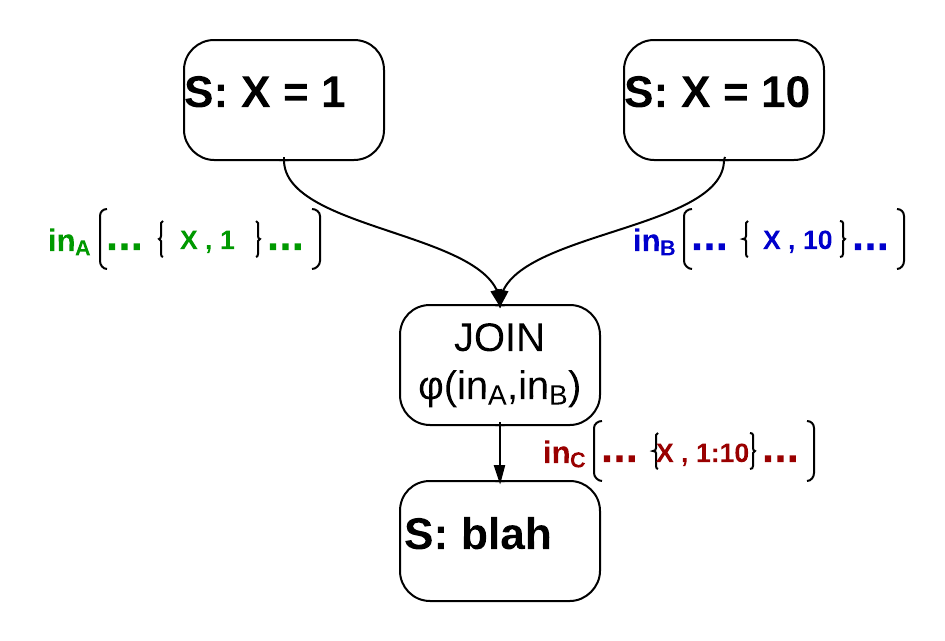
\includegraphics[width=0.4\textwidth]{MergeNode}
\caption{A Range analysis merge. Unlike constant propagation, $x$ becomes all possible values at $in_c$ and not top. }
\label{RngMergeNode}
\end{figure}
There are two complications with this analysis which are described as follows;\\
\begin{itemize}
\item{\textbf{Flow functions:} Flow functions must assume range tuples and calculate the maximum tuple for each statement.}
\item{\textbf{Loop detection:} Given that the range of numbers is infinite, for termination a heuristic loop detector should be added to the join. We will elaborate later in the document.}
\end{itemize}
\subsection{Lattice \& Flow Functions}
for range analysis, we decompose all variable types to two numerical primitives of \emph{int} and \emph{float} that correspond to LLVM's constant and register types \emph{IntxTy} and \emph{FloatTy}. This bounds range to the \emph{max} and \emph{min} of these types, but it is still large enough that we need the heuristic loop detector mentioned earlier. Any constant or operand that cannot be cast to a \emph{int} or \emph{float} cannot have a range and so will be outside of the lattice domain.\\
We introduce the concept of:
$$ X \ra \{min,max\} \in Z^2$$
to represent the range of a variable $X$ given the set of variables $Z$, where $min$ is the lowest value X could be and $max$ is the highest. \\
Furthermore we define all constants $N$ to be a range of 1 using similar notation: 
$$ N \ra\{n,n\} \in \mathbb{R}$$
This means that constants may be assigned to variables, as is necessary for analysis and in actual code. \\
\subsubsection{Lattice and the Join}
The set join is complicated for range analysis so extra discussion is provided after defining the lattice.
Let $Vars$ be the set of C++ variables present in the program. Given two flows $F,F'$, we have :
\begin{align*}
F \sqsubseteq & F'  & \lra & & F \subseteq F' \\
\top & & \lra & & \{ X \ra \{-\infty; +\infty\} | \forall X \in Vars \}\\ 
\bot & & \lra & & \emptyset \\ 
F \sqcup F' & & \lra & & (F \ra h(F)) \cup (F'\ra h(F')) \\
F \sqcap F' & & \lra & & F \cap F'
\end{align*}

\textbf{The Join}\\
$h(X)$ is a loop detection heuristic. 
\begin{figure}[here]
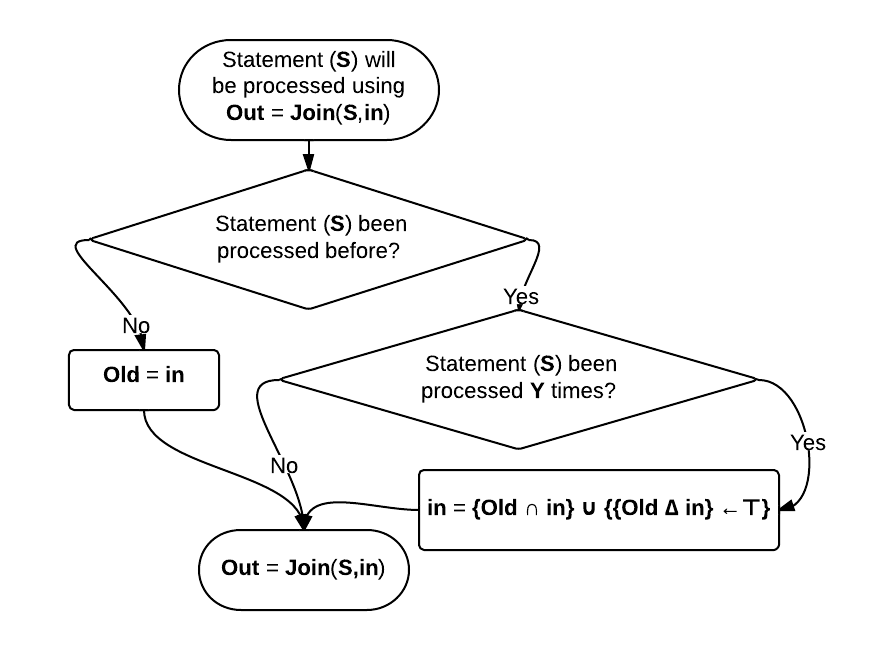
\includegraphics[width=0.4\textwidth]{loopDetector}
\caption{The range analysis Join. A heuristic is used to quickly reach a fixed point for the loop body statements.}
\label{LoopDetectHeuristic}
\end{figure}

The heuristic is described a flow chart in Figure~\ref{LoopDetectHeuristic}
The heuristic can guarantee correctness but depending on Y it may can give very imprecise information. A higher $Y$ increasing the likelihood the loop control will reach its upper bound, which increases precision since a local fixed point occurs and statements from the loop body will not be added to the work list at this point. We were not aggressive with $Y$ because of an exponential analysis run-time cost. We reason a cost factor of $\bar{Loops} \times \bar{BodyLength}$ meaning $Y$ should not be too high for scalable analysis and choose 3 to demonstrate our heuristic concept. We considered a more sophistic range detection based on taken/untaken predecessor blocks, but unable to successfully implement this. More detail is provided in the implementation section.

\subsubsection{Flow Functions}
We list the instructions covered by our our range analysis in Table~\ref{rangeAnalysisTable}. For each instruction, we define $F_{IN}$ and $F_{OUT}$ as the input and output of the flow functions for each instruction, respectively. Table~\ref{rangeAnalysisTable} is a selection of flow functions to show the supported binary arithmetic and logical statements of our range analysis. We do not list a flow function for every operand type permutation (possible operand combinations of constants, $N$ and variables $X$). We do not need to do so since constants and variables exist in our domain ($\bot \subseteq n \subseteq \top \forall N$ and $\bot \subseteq x \subseteq \top \forall X$) so either $A$ or $B$ or both in Table~\ref{rangeAnalysisTable} may be substituted with $N$. For the same reason we also do not list different flow functions for The primitive types \emph{FloatTy} and \emph{IntxTy}. The flow functions all use a binary operator substitution, \emph{Combo(A,B,Op)} defined under Table~\ref{rangeAnalysisTable} to exhaustively find the maximum range of any binary operator. This could be optimized for adding and shifting cases, but we feel this would obfuscate the flow functions.\\
Besides the binary operators we define flow functions for pointer de-reference. Because our pass has no access to points-to information, to be safe our pass simply returns max range to either the assigned variable or the set of variables.  %All upper case literals are variables and all lower case literals are constants. We use shorthand for readability of our flow functions, which is expanded below the main table. 
%{\footnotesize
%\begin{align*} 
%& X \la A + B  & : & & F_{OUT} = F_{IN} - \{X \ra *\}\cup \{ X \ra \{min(Combo(A,B,+)); max(Combo(A,B,+)) \} | A \in Vars \wedge B \in Vars \} \\
%& X \la A - B & : & & F_{OUT} = F_{IN} - \{X \ra *\}\cup \{ X \ra \{min(Combo(A,B,-)); max(Combo(A,B,-)) \} | A \in Vars \wedge B \in Vars \} \\
%& X \la A \times B & : & & F_{OUT} = F_{IN} - \{X \ra *\}\cup \{ X \ra \{min(Combo(A,B,\times)); max(Combo(A,B,\times)) \} | A \in Vars \wedge B \in Vars \} \\
%& X \la A \div B & : & & F_{OUT} = F_{IN} - \{X \ra *\}\cup \{ X \ra \{min(Combo(A,B,\div)); max(Combo(A,B,\div)) \} | A \in Vars \wedge B \in Vars \} \\
%& X \la A MOD B & : & & F_{OUT} = F_{IN} - \{X \ra *\}\cup \{ X \ra \{min(Combo(A,B, \%)); max(Combo(A,B,\%)) \} | A \in Vars \wedge B \in Vars \} \\
%& X \la A LSHL B & : & & F_{OUT} = F_{IN} \cup \{W \ra Z | X \ra W \wedge Y \ra Z \} \\
%& X \la A LSHR B & : & & F_{OUT} = F_{IN} \cup \{X \ra Z | Y \ra W \wedge W \ra Z \} \\ 
%& X \la A ASHR B & : & & F_{OUT} = F_{IN} \cup \{X \ra Z | Y \ra W \wedge W \ra Z \} 
%\end{align*}

%where:
%}%

\begin{table*}[t]
\centering
\caption{Range analysis flow functions}
\begin{tabular}{| c | l | }
\hline
\multicolumn{1}{c}{\textbf{Statement}} & 
  \multicolumn{1}{c}{\textbf{Flow function}}\\\hline
$X \la A + B$  & \shortstack{$F_{OUT} = F_{IN} - \{X \ra *\}\cup$ \\$\{ X \ra \{min(Combo(A,B,+)); max(Combo(A,B,+)) \} | A \in Vars \wedge B \in Vars \}$} \\
$X \la A - B$  & \shortstack{$F_{OUT} = F_{IN} - \{X \ra *\}\cup$ \\$\{ X \ra \{min(Combo(A,B,-)); max(Combo(A,B,-)) \} | A \in Vars \wedge B \in Vars \}$} \\
$X \la A \times B$  & \shortstack{$F_{OUT} = F_{IN} - \{X \ra *\}\cup$ \\$\{ X \ra \{min(Combo(A,B,\times)); max(Combo(A,B,\times)) \} | A \in Vars \wedge B \in Vars \}$} \\
$X \la A \div B$  & \shortstack{$F_{OUT} = F_{IN} - \{X \ra *\}\cup$ \\$\{ X \ra \{min(Combo(A,B,\div)); max(Combo(A,B,\div)) \} | A \in Vars \wedge B \in Vars \}$} \\
$X \la A \% B$  & \shortstack{$F_{OUT} = F_{IN} - \{X \ra *\}\cup$ \\$\{ X \ra \{min(Combo(A,B,\%)); max(Combo(A,B,\%)) \} | A \in Vars \wedge B \in Vars \}$} \\
$X \la A LSHL B$  & \shortstack{$F_{OUT} = F_{IN} - \{X \ra *\}\cup$ \\$\{ X \ra \{min(Combo(A,B,LSHL)); max(Combo(A,B,LSHL)) \} | A \in Vars \wedge B \in Vars \}$} \\
$X \la A LSHR B$  & \shortstack{$F_{OUT} = F_{IN} - \{X \ra *\}\cup$ \\$\{ X \ra \{min(Combo(A,B,LSHR)); max(Combo(A,B,LSHR)) \} | A \in Vars \wedge B \in Vars \}$} \\
$X \la A ASHR B$  & \shortstack{$F_{OUT} = F_{IN} - \{X \ra *\}\cup$ \\$\{ X \ra \{min(Combo(A,B,ASHR)); max(Combo(A,B,ASHR)) \} | A \in Vars \wedge B \in Vars \}$} \\
$X \la *Y$ & $F_{OUT} = F_{IN} - \{X \ra *\}\cup \{X \ra \{-\infty,+\infty\}\}$\\
$*X \la Y$ & $F_{OUT} = F_{IN} - \{Z \ra * \forall Z\in Vars\}\cup \{Z \ra \{-\infty,+\infty\} \forall Z\in Vars\}\}$\\
\hline

\end{tabular}
\label{rangeAnalysisTable}

where: ${M[m_1:m_4]} \gets Combo(A,B,Op) \lra ((A_{[0]} Op B_{[0]}),(A_{[0]} Op B_{[1]}),(A_{[1]} Op B_{[0]}),(A_{[1]} Op B_{[1]}))$ 
\end{table*}

%Notice that scope of instructions covered could be larger and these out-of-scope instructions fall into two categories. Instructions such as $X \la c$ (where $X$ is a pointer variable) are explicitly forbidden in C++ language. Instructions such as $*X \ra *Y$ are legitimate candidates but where not implemented because of time constraints. 
\subsection{Implementation}
The range analysis pass is performed after a "\textbf{mem2reg}" pass. Without mem2reg, the pass must resolve variables from load and store instructions along with other complications.\\
Using mem2reg has a disadvantage that source code variables do not correspond to the .ll code input to our range analysis. We were unable to robustly transpose source code variables to our range analysis input, so our range analysis could not implement bounds checking.\\
Because of this limitation we were not aggressive with our join heuristics and chose a simple three statement counter to demonstrate the concept of heuristic loop detection for balancing pass execution time and information preciseness.\\
We provide an example snipped  for a flow function but focus discussion on our join operator. This is because our flow functions follow a similar template and because the join heuristic is responsible for a practical range analysis' achievable precision.\\
The multiplication flow function is as follows:
%Each mathematical instruction is identified by its corresponding C++ and LLVM code snippets, which are available on table \ref{pointerAnalysisTable}. When the \code{Flow* executeFlowFunction()} is executed, the instruction's opcode is parsed and the computation performed is selected using switch statements as follows :

\begin{lstlisting}[caption=Range analysis flow functions, label=PAFF]
DomEl getOpRng(DomEl a, 
               DomEl b, 
               unsigned opcode)
{
...//Declarations, sanity checks etc.
  switch(opcode) 
  {
  	...
    case MUL:

      Comb[0] = a.lower * b.lower;
      Comb[1] = a.lower * b.upper;
      Comb[2] = a.upper * b.lower;
      Comb[3] = a.upper * b.upper;
      resRange.lower = Comb[0];
      resRange.upper = Comb[0];
      while(i < 4)
      {
        if(Comb[i] < resRange.lower)
    	         resRange.lower = Comb[i];
        if(Comb[i] > resRange.upper)
    	         resRange.upper = Comb[i];
        i++;
      }
      break;
    ...
  }//end case
  return resRange;
}
\end{lstlisting}

The Join operation is composed of three parts:
\begin{itemize}
\item{\textbf{Heuristic loop detection $h(in)$: }Keep copies of the first mappings for each statements. Output is consumed by the join operation.}
\item{\textbf{Join sets $\cup$: }The set wise join operation}
\item{\textbf{Join elements: }A range analysis specific element wise join taking the maximum possible range of two domain elements}
\end{itemize}

Besides the set join, $\cup$, we provide code snippets below. Set join is omitted since it is similar to other analysis.\\

\jules{Jules : not sure if those listings are useful. Could help us save one page.}
 \begin{lstlisting}[caption=Heuristic loop detector $h(in)$, label=PAFF]
Flow* FF(Flow *in, Ins *inst, int S_id) 
{
 if(nodeCount.find(S_id)!=nodeCount.end())
 {
    //Y is set to 3
    if(nodeCount[S_id].VisitCtr >= 3)
    {
      ...
      //Set ranges that changed to TOP
      DifToTop(in, 
               nodeCount[S_id].nodeSet);
      //*in is modified
      return(in);
    }
    nodeCount[S_id].VisitCtr = 
              (nodeCount[S_id].VisitCtr+1);
  }
  else
  {
    ...
    nodeState thisNodeState;
	thisNodeState.VisitCtr = 1;
	thisNodeState.nodeSet = in;//'Old'
	nodeCount[NodeId] = thisNodeState;
  }

 \end{lstlisting}
 
 \begin{lstlisting}[caption=Per domain element join, label=PAFF]
DomEl JoinEls(DomEl* A, DomEl* B)
{
  DomEl maxAB;

  maxAB.lower = (A->lower <= B->lower) ? 
                       A->lower : B->lower;
  maxAB.upper = (A->upper >= B->upper) ? 
                       A->upper : B->upper;
  return maxAB;
}
 \end{lstlisting}